\documentclass{article}
\usepackage[utf8]{inputenc}
\usepackage[T1]{fontenc}
\usepackage{graphicx}
\usepackage{indentfirst}
\usepackage{fancyhdr}
\usepackage[a4paper,left=2cm,right=2cm,top=2.5cm,bottom=2cm]{geometry}
\usepackage{amsmath}
\usepackage{amssymb}
\usepackage{array}
\usepackage{pifont}
\usepackage{makecell}
\usepackage{xcolor}
\newcommand{\tabitem}{~~\llap{\ding{213}}~~}
\definecolor{pythonColor}{HTML}{B634F6}
\newcommand{\python}[1]{\textcolor{pythonColor}{\textit{#1}}}

% Propriétés de la matrice A:
%     Test à faire : ({Real, complex},
%                     {Pleine, Creuses{Bandes, Pas bandes}},
%                     {Symétrique} )


% Paramètres infuençant le conditionnement
%     SICN  : signed inverse condition number
%     SIGE  : signed inverse gradient error
%     Gamma : vol/sum_face/max_edge

\title{Analyse numérique : Homework 1}
\author{Romain Graux}
\date{Monday, 14 October 2019}

\begin{document}
\maketitle

\section{Propriétés de la matrice \textit{A}}

Ces données ont été obtenues par le biais de la fonction \python{all\_test}\textit{()} contenue dans le ficheir \textit{mysolve.py}. Tous les tests ont été fait sur un raffinement tel que \python{ref}$ = 0.05$, ce qui correspond à \textit{1138} éléments.

\begin{center}
\begin{tabular}{|p{1cm}|p{4cm}|p{4cm}|}
    \hline
    & \makecell{\textit{freq$=$0}}      & \makecell{\textit{freq$\neq $0}} \\
    \hline
    \makecell{\textit{vel$=$0}}
    & \makecell{\textbf{Statique}}      & \makecell{\textbf{Harmonique}} \\
    &                                   &                                \\
    & Réelle                            & Complexe                       \\
    & Symétrique                        & Symétrique                     \\
    & Définie positive                  & Définie positive               \\
    & Creuse ($\cong 3\%$)              & Creuse ($\cong 3\%$)           \\
    & Hermitienne                       & Non hermitienne                \\
    & Inversible                        & Inversible                     \\
    &                                   &                                \\
    \hline
    \makecell{\textit{vel$\neq $0}}
    & \makecell{\textbf{Stationnaire}}  & \makecell{\textbf{Dynamique}}  \\
    &                                   &                                \\
    & Réelle                            & Complexe                       \\
    & Non symétrique                    & Non symétrique                 \\
    & Non définie                       & Non définie                    \\
    & Creuse ($\cong 3\%$)              & Creuse ($\cong 3\%$)           \\
    & Non hermitienne                   & Non hermitienne                \\
    & Inversible                        & Inversible                     \\
    &                                   &                                \\
    \hline
\end{tabular}
\end{center}

\section{Paramètres influençant le conditionnement de \textit{A}}
\subsection{Largeur de l'entrefer}
\begin{center}
    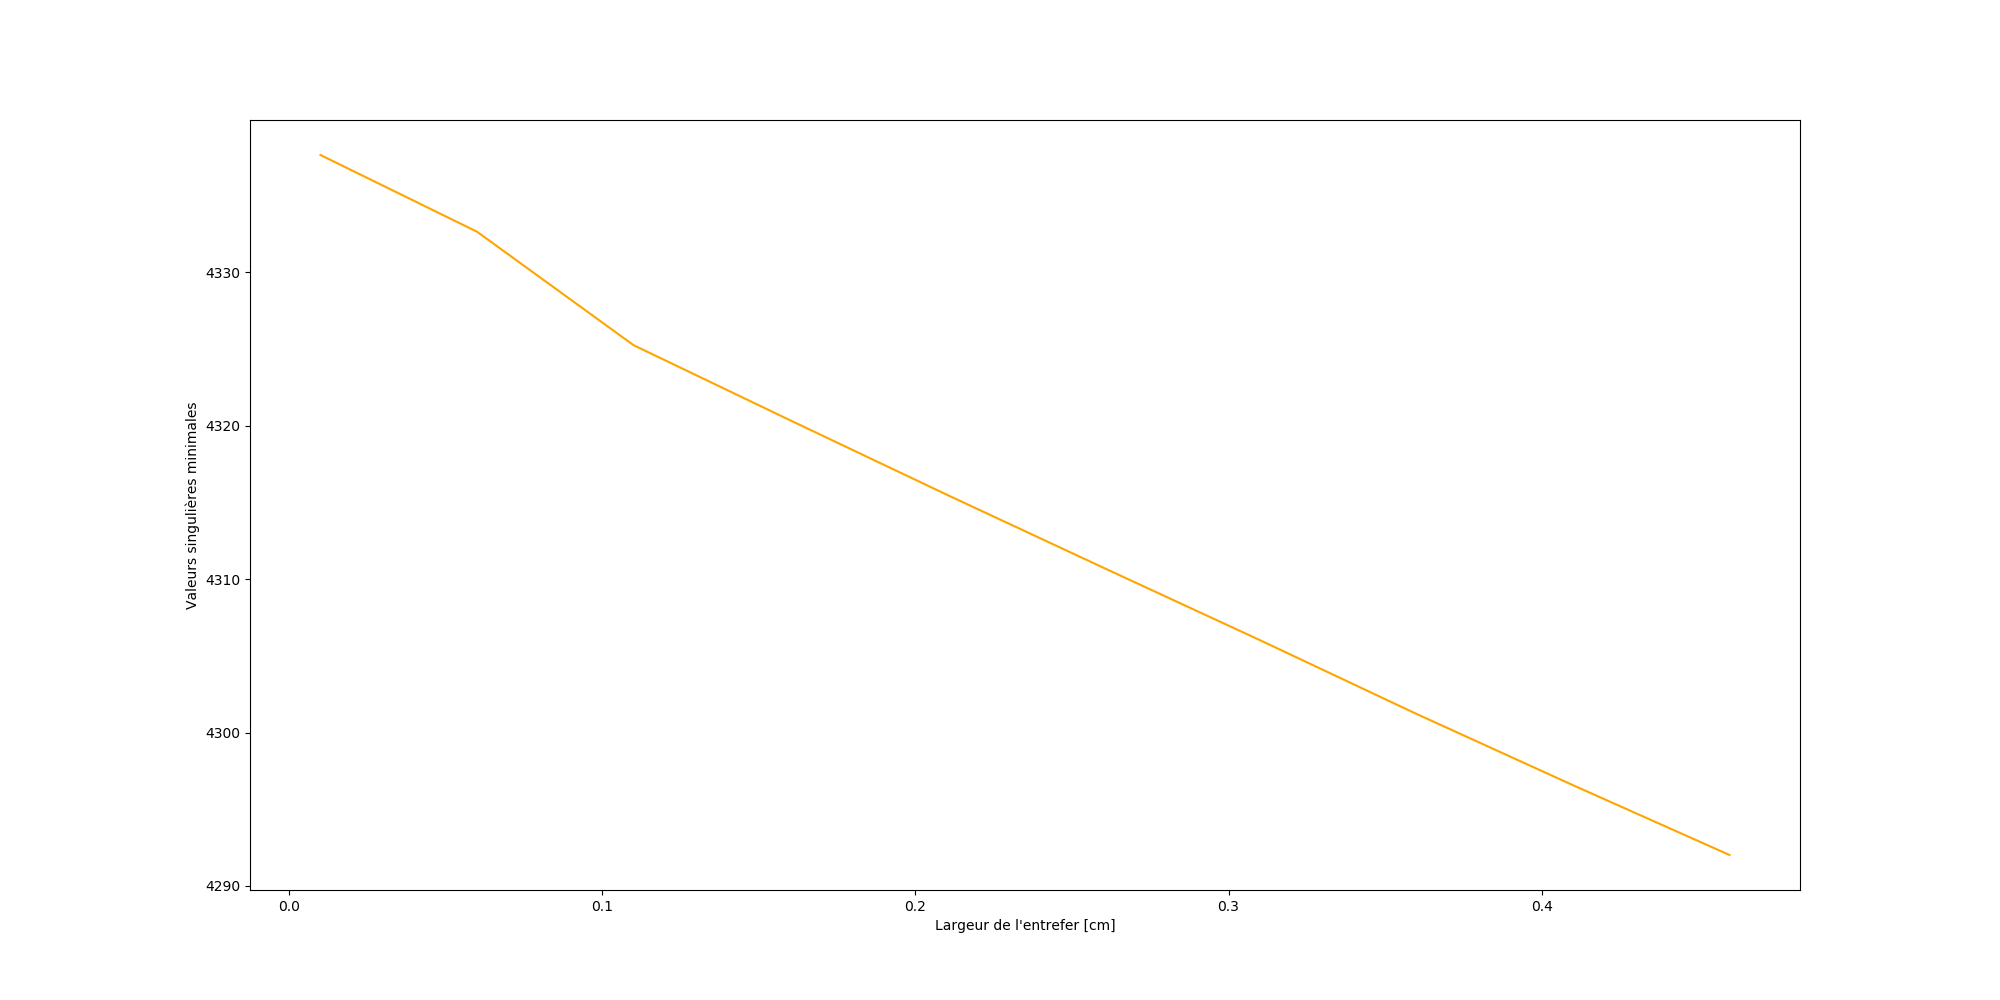
\includegraphics[width = 10cm]{influences/plots/gap_min.png}
    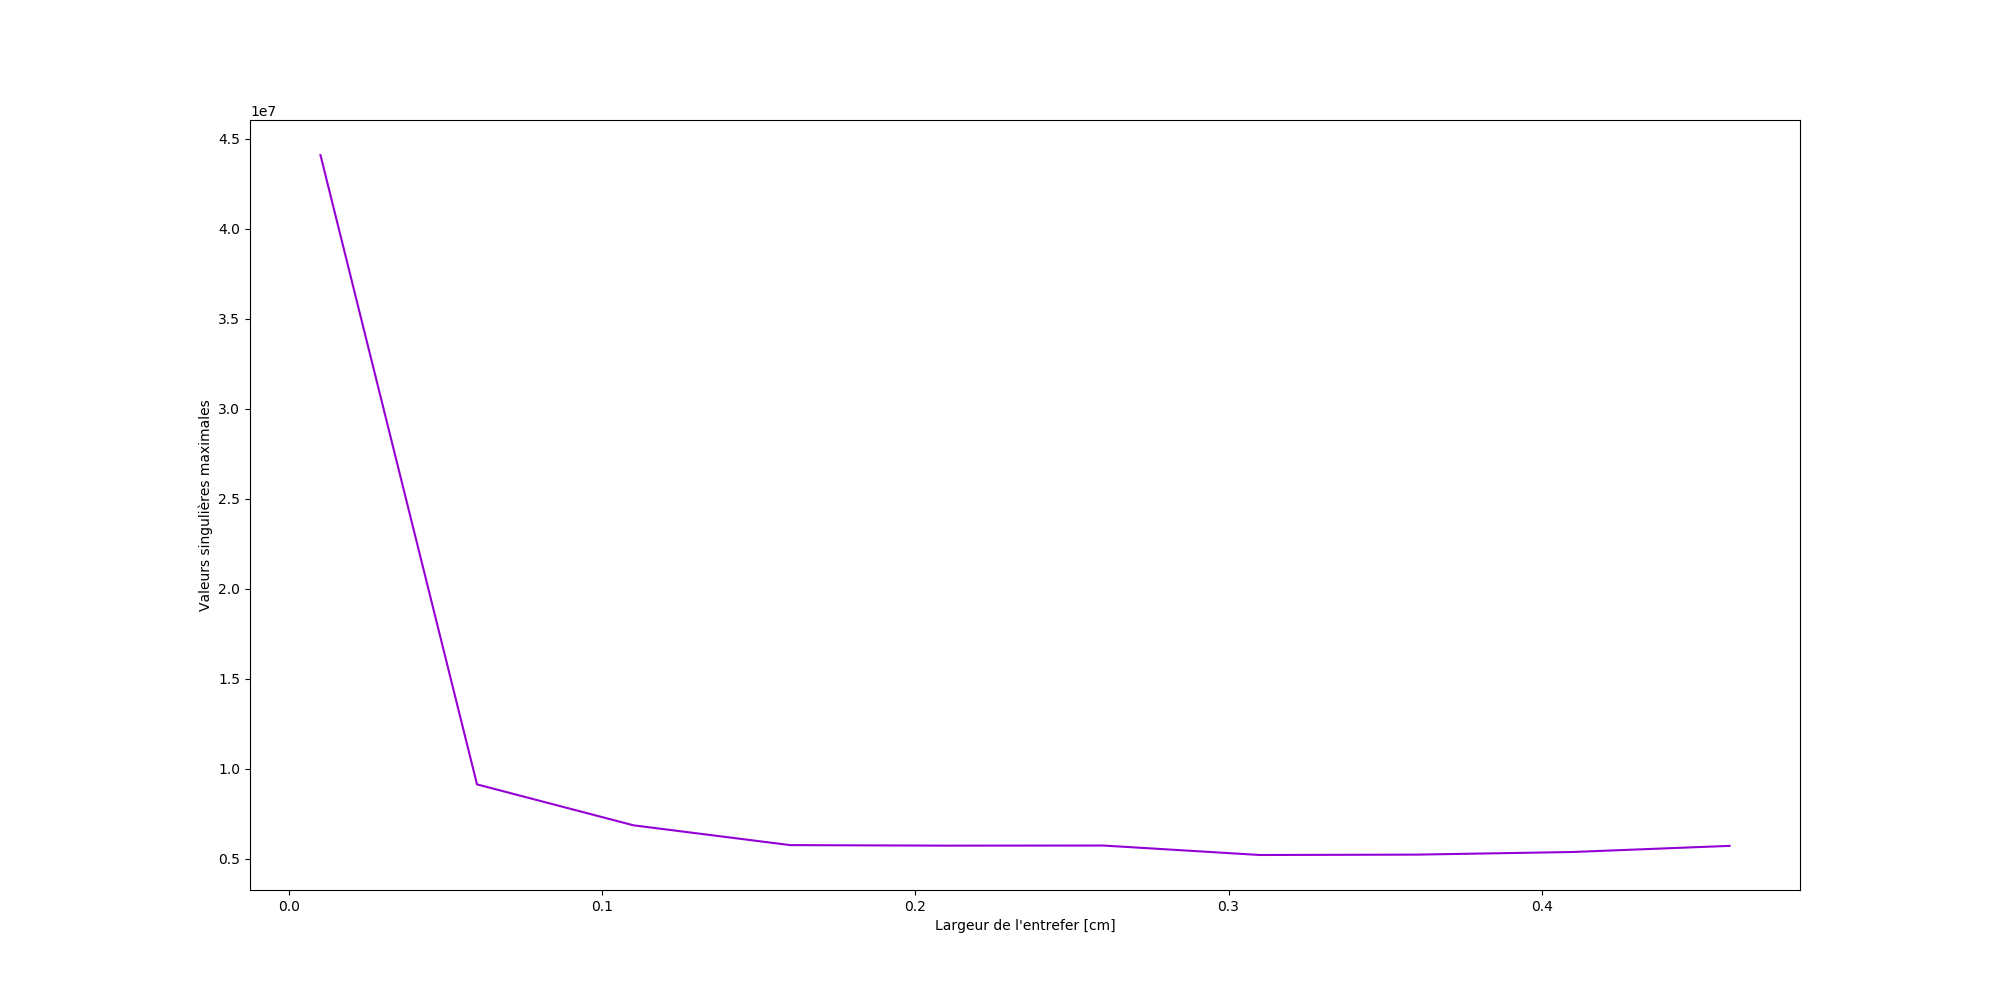
\includegraphics[width = 10cm]{influences/plots/gap_max.png}
    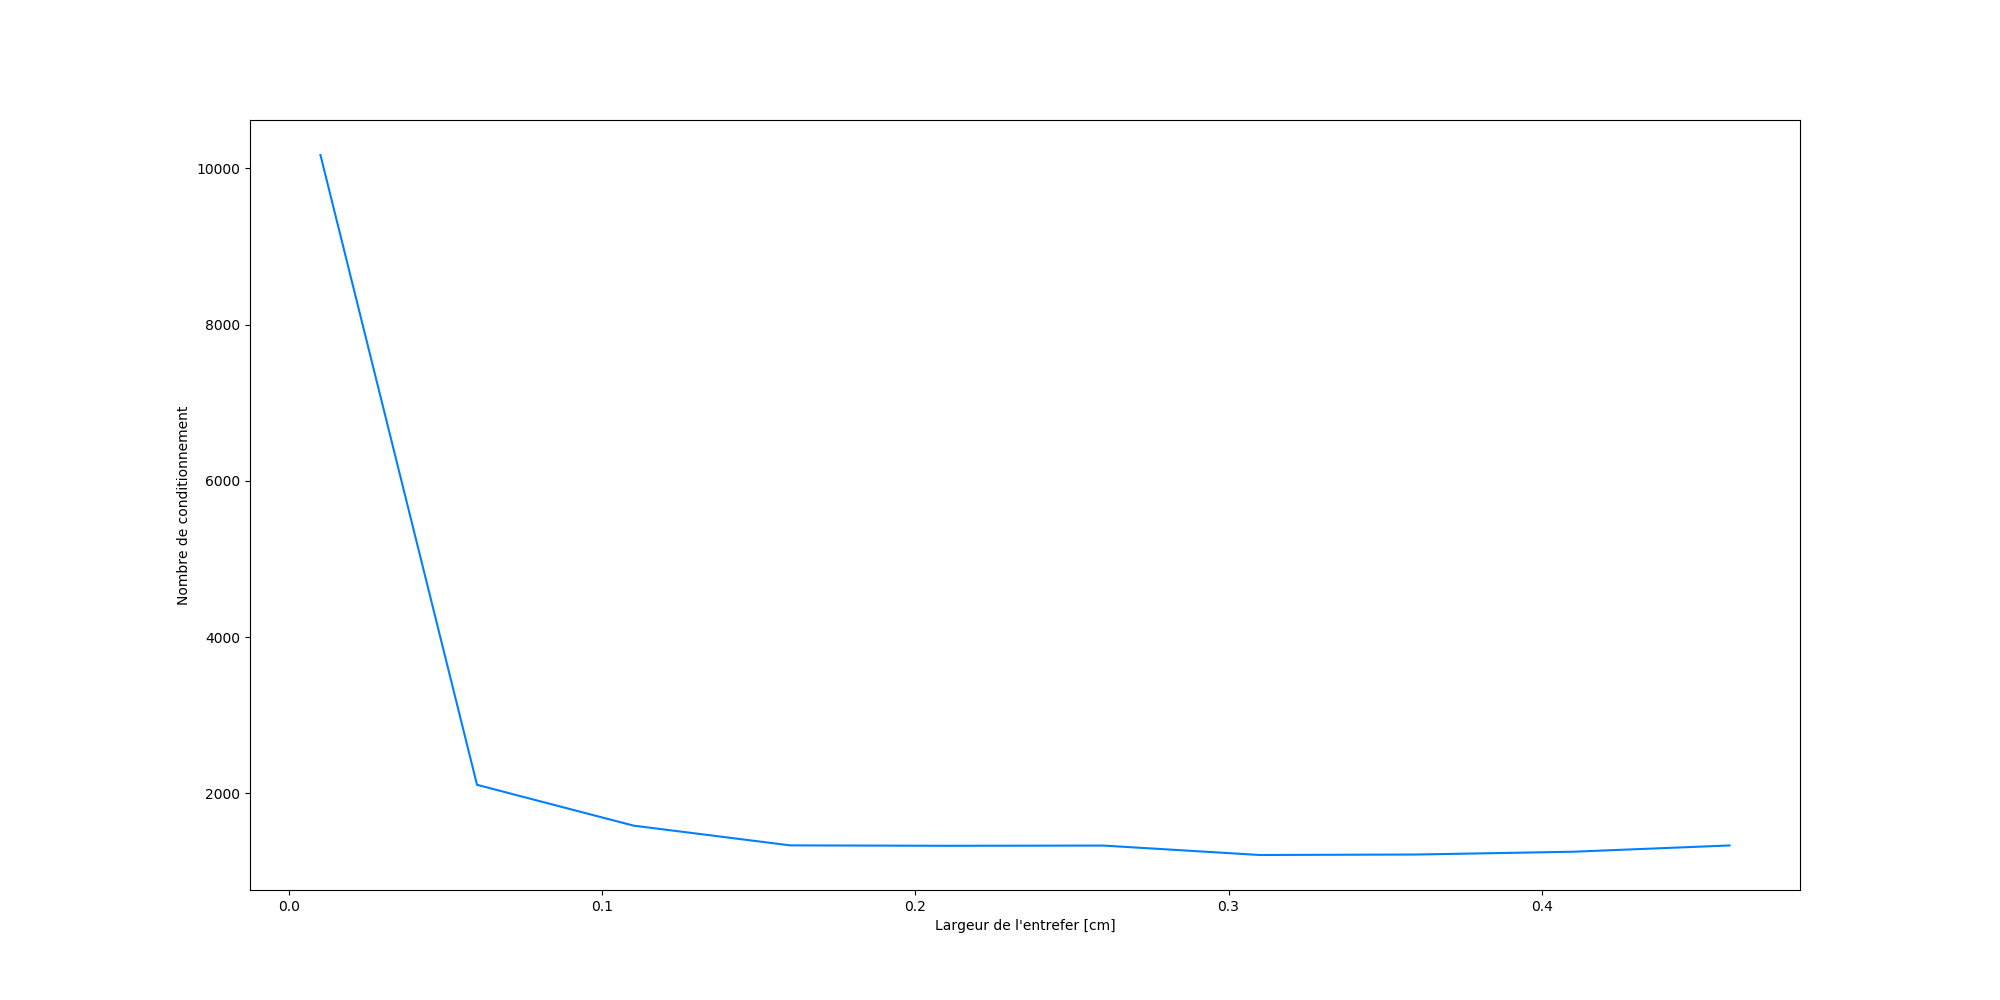
\includegraphics[width = 10cm]{influences/plots/gap_k.png}
\end{center}

\subsection{Perméabilité relative}
\begin{center}
    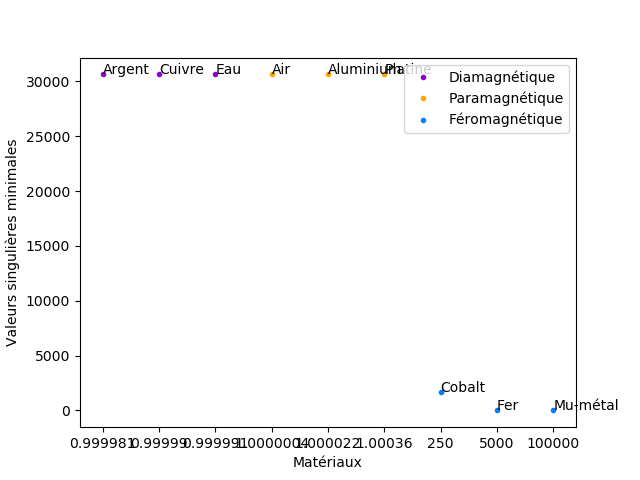
\includegraphics[width = 10cm]{influences/plots/perm_min.png}
    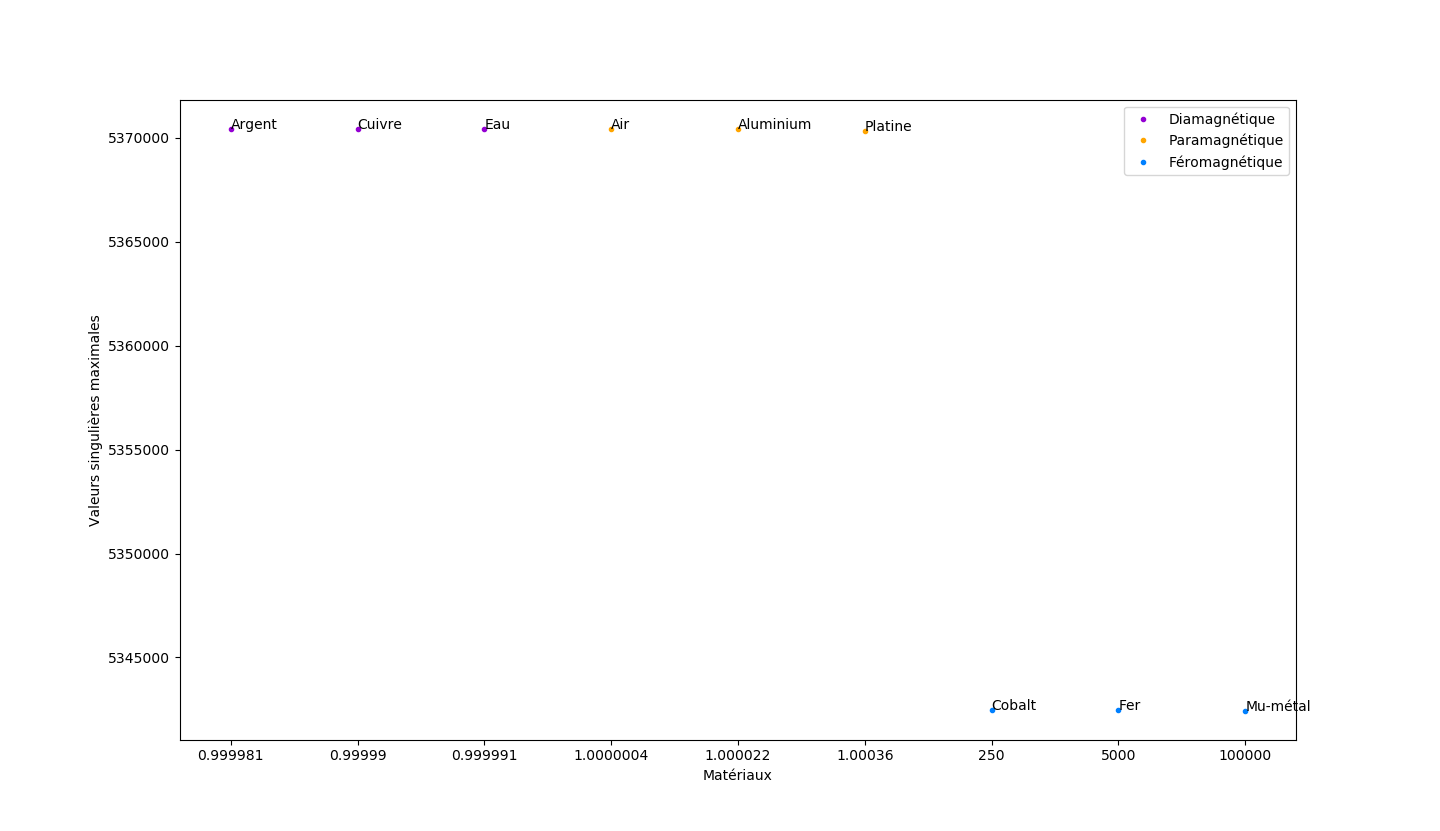
\includegraphics[width = 10cm]{influences/plots/perm_max.png}
    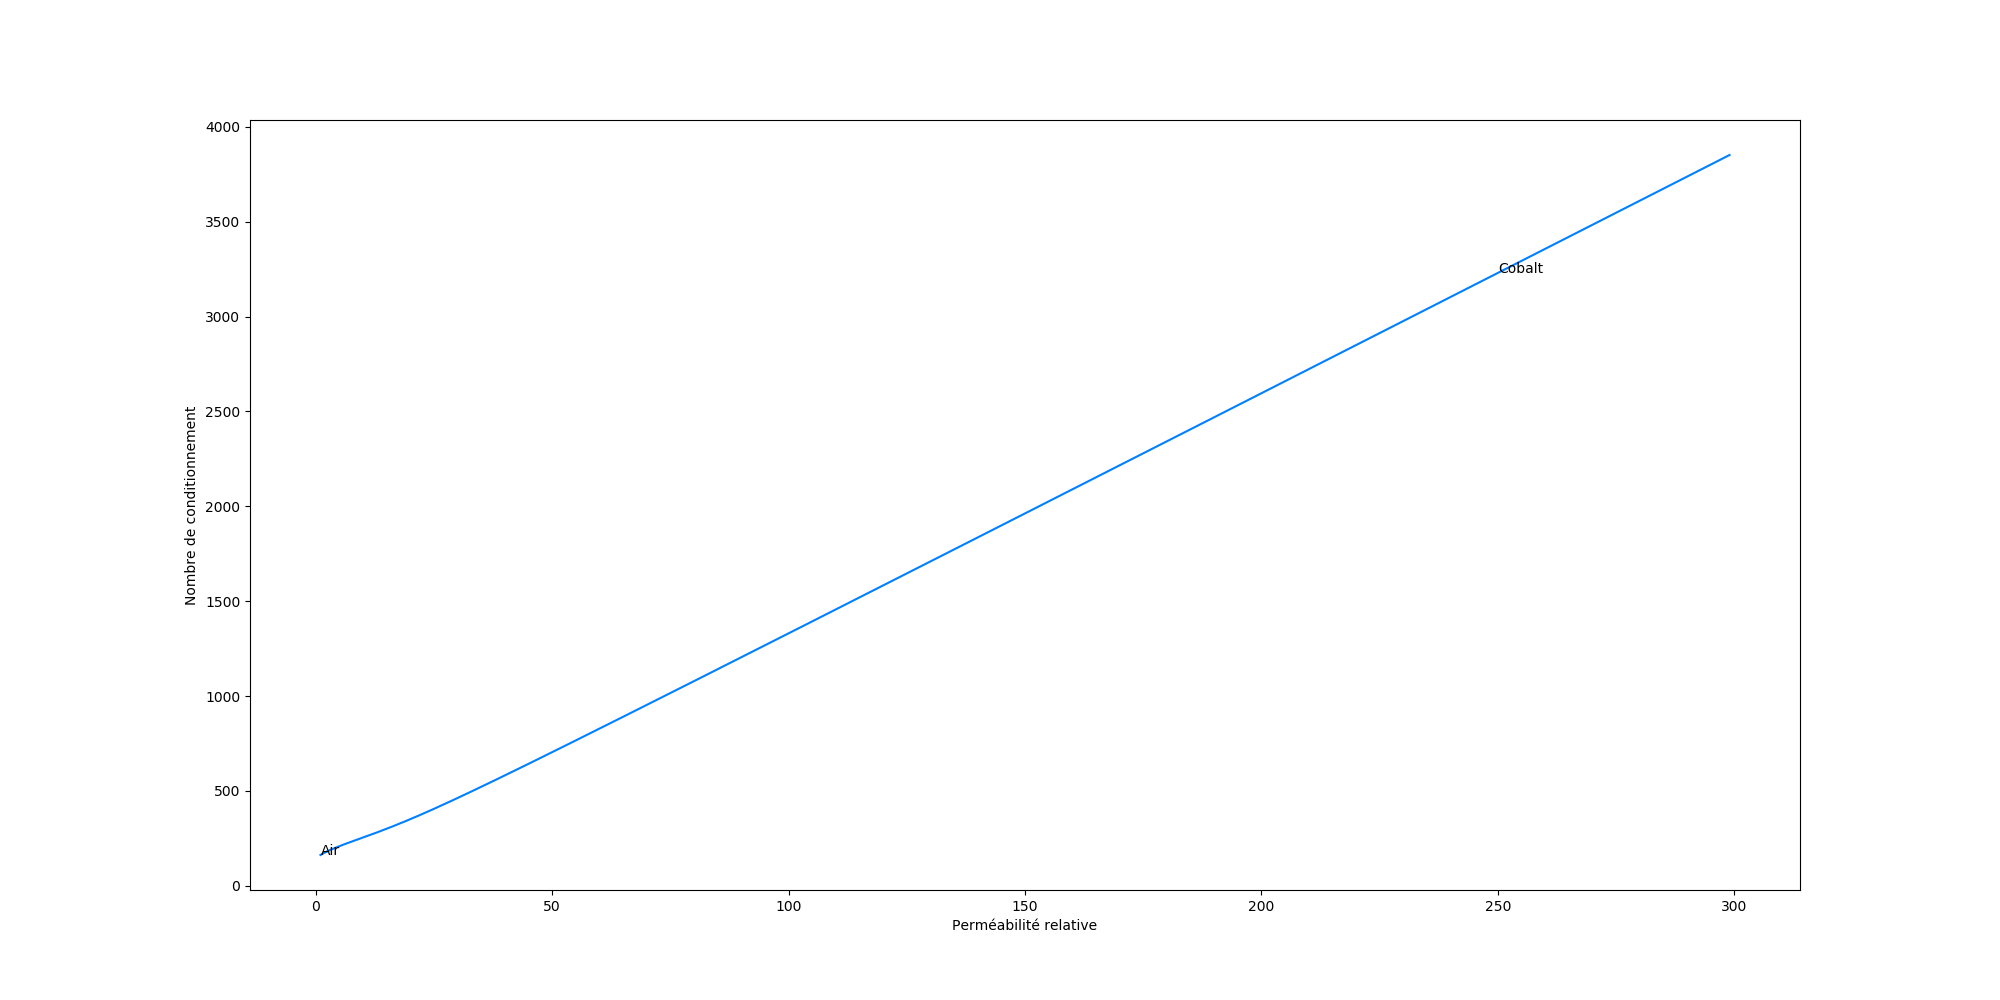
\includegraphics[width = 10cm]{influences/plots/perm_k.png}
\end{center}

\subsection{Maillage}
\begin{center}
    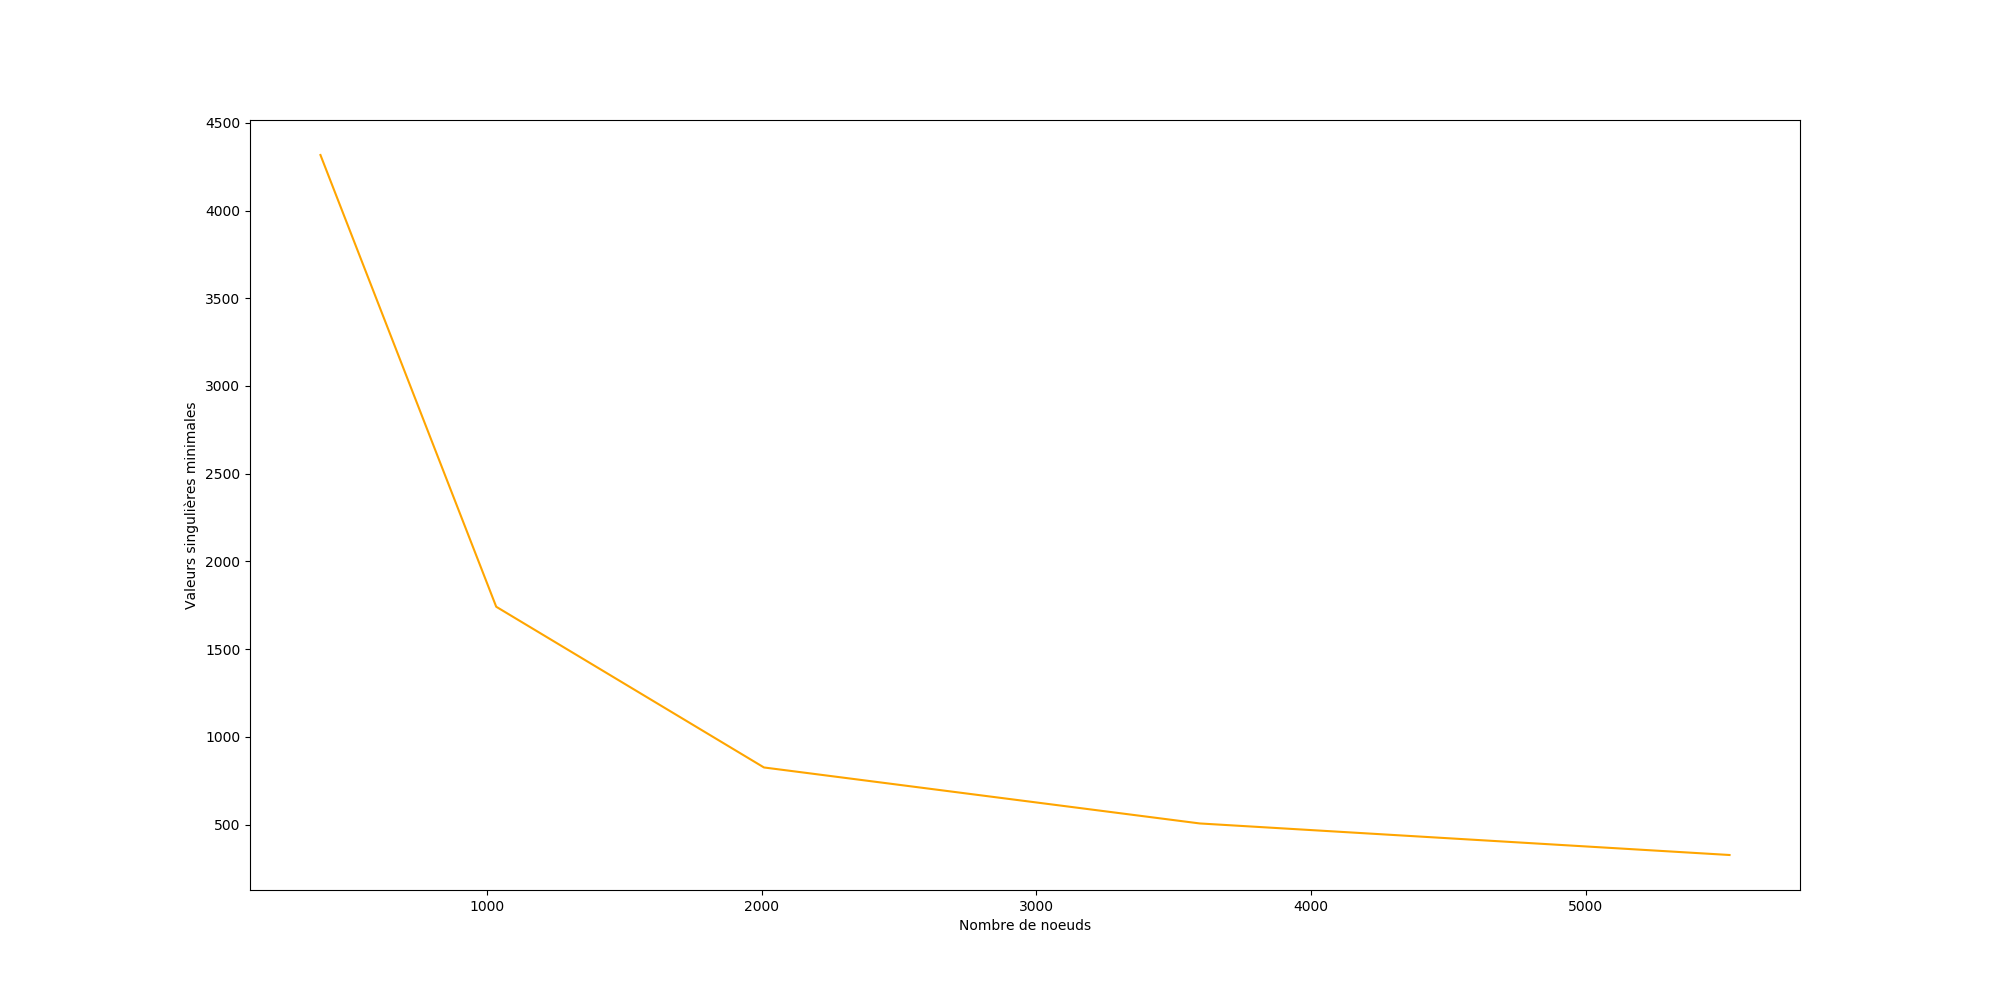
\includegraphics[width = 10cm]{influences/plots/ref_min.png}
    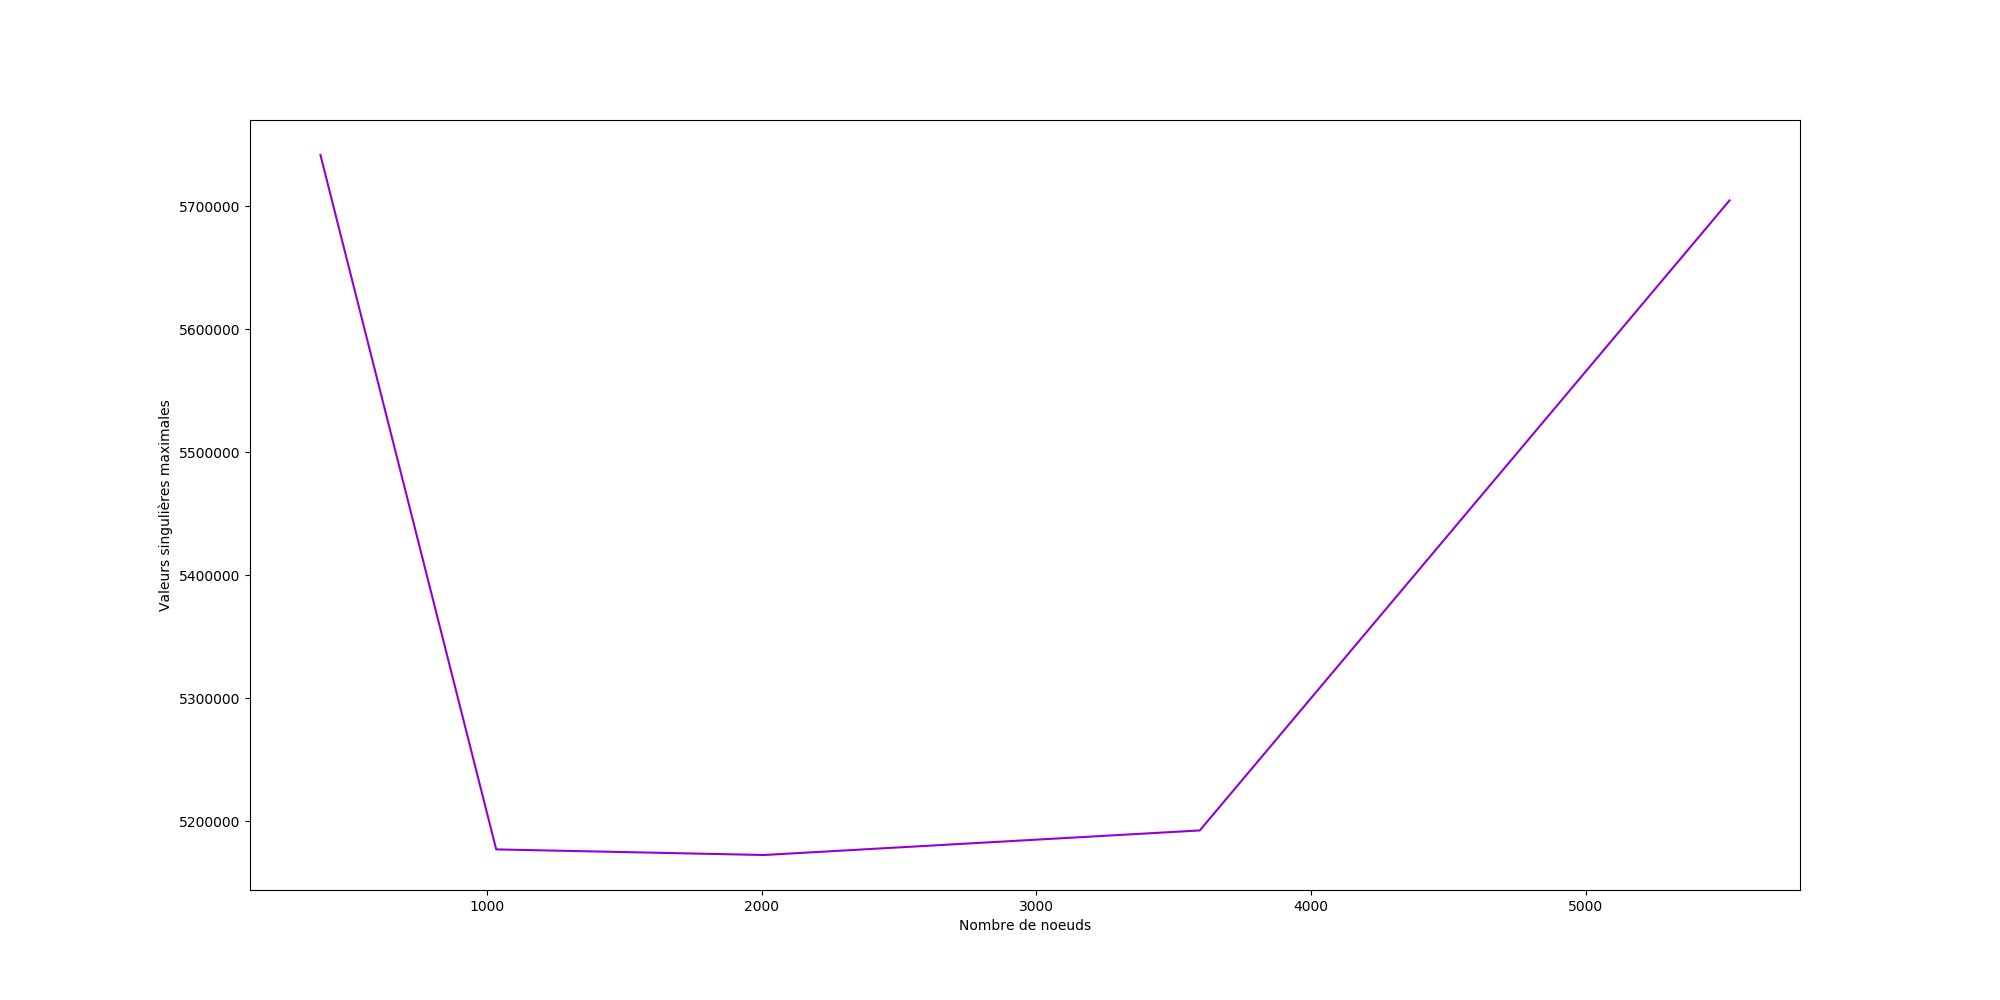
\includegraphics[width = 10cm]{influences/plots/ref_max.png}
    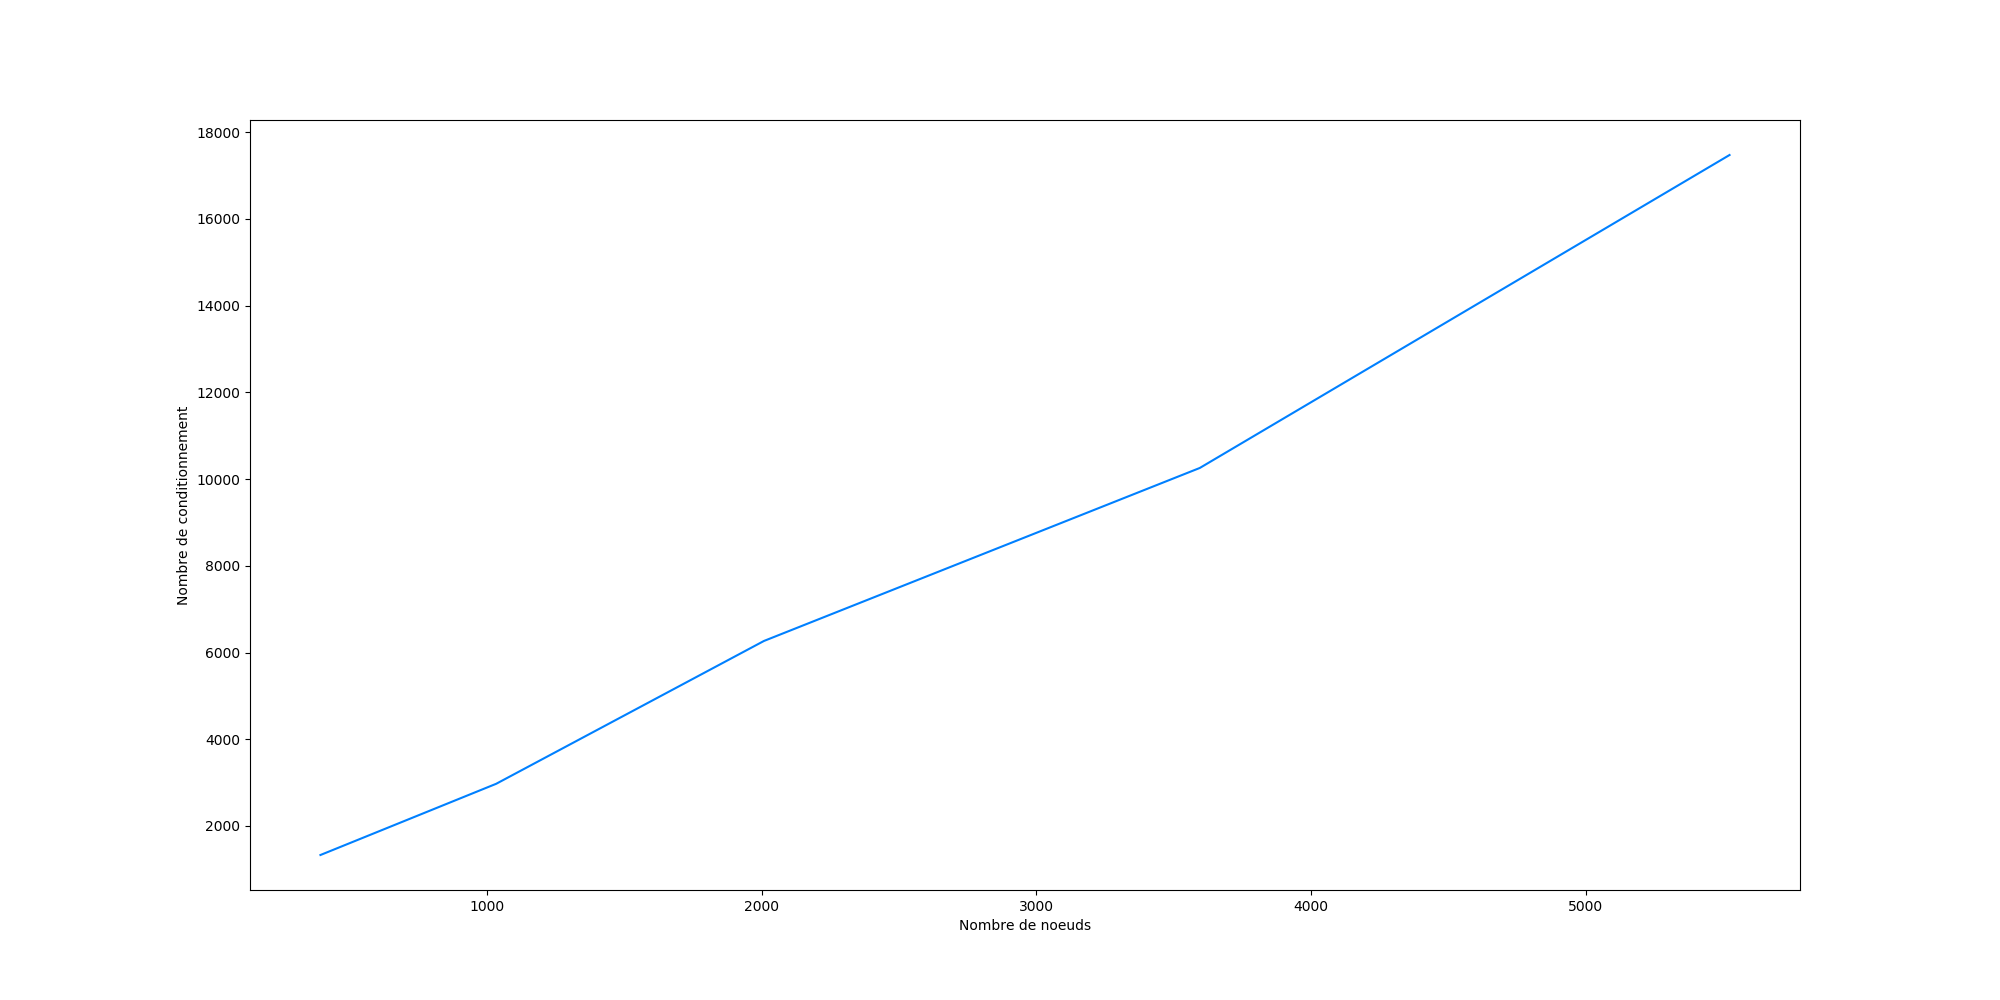
\includegraphics[width = 10cm]{influences/plots/ref_k.png}
\end{center}

\section{Interprétation}

\end{document}
